% SPDX-License-Identifier: CC-BY-SA-4.0
% Author: Matthieu Perrin
% Part: <Nom de la partie>
% Section: <Nom de la section>
% Sub-section: <Nom de la sous-section>  % (facultatif, laisser vide si non utilisé)
% Frame: <Titre de la slide>

\begingroup

\begin{frame}{Un exemple : le \og Subset-Sum Problem\fg}
    Existe-t-il un sous-ensemble non-vide de nombres dont la somme est $0$ ? 

  \vspace{2mm}
  \begin{center}
    \scalebox{1.1}{
    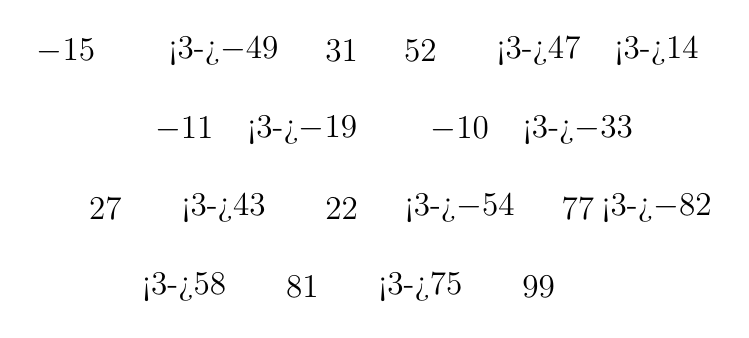
\begin{tikzpicture}
      \draw (5,3) node  {\large $31$};
      \draw (2,1) node  {\large $27$};
      \draw (3,2) node  {\large $-11$};
      \draw (4.5,0) node  {\large $81$};
      \draw (5,1) node  {\large $22$};
      \draw (6.5,2) node  {\large $-10$};
      \draw (7.5,0) node  {\large $99$};
      \draw (8,1) node  {\large $77$};
      \draw (1.5,3) node {\large $-15$};
      \draw (6,3) node  {\large $52$};
      \draw (7.5,3) node  {\large \alert<3->{$47$}};
      \draw (9,1) node  {\large \alert<3->{$-82$}};
      \draw (3,0) node  {\large \alert<3->{$58$}};
      \draw (3.5,1) node  {\large \alert<3->{$43$}};
      \draw (4.5,2) node  {\large \alert<3->{$-19$}};
      \draw (6,0) node  {\large \alert<3->{$75$}};
      \draw (6.5,1) node  {\large \alert<3->{$-54$}};
      \draw (8,2) node  {\large \alert<3->{$-33$}};
      \draw (9,3) node {\large \alert<3->{$14$}};
      \draw (3.5,3) node  {\large \alert<3->{$-49$}};
    \end{tikzpicture}}
  \end{center}

  \pause
  \begin{block}{Solution}
    \begin{itemize}
    \item<2-> La réponse est oui
    \item<3-> $47-82+58+43-19+75-54-33 + 14 -49 = 0$
      \begin{itemize}
      \item On ajoute un \structure{certificat polynomial} pour permettre la vérification
      \end{itemize}
    \end{itemize}
  \end{block}
\end{frame}
\endgroup
